\documentclass{beamer}

%\usepackage{lmodern}
\usepackage[font=scriptsize,skip=0pt,justification=justified,singlelinecheck=false]{caption}
%\usepackage{enumitem}
\usepackage{natbib}
\usepackage{bm}
\usepackage{mathtools}
\usepackage[makeroom]{cancel}


% Insert a Video
\usepackage{multimedia} 

% Using underline
\usepackage{soul}


%remove the icon
\setbeamertemplate{bibliography item}{}

%remove line breaks
\setbeamertemplate{bibliography entry title}{}
\setbeamertemplate{bibliography entry location}{}
\setbeamertemplate{bibliography entry note}{}
% Use number for caption
\setbeamertemplate{caption}[numbered]{}

\newtheorem{mydef}[theorem]{\Large \underline{\textbf{Definisi}}}

\makeatletter
\def\th@mystyle{%
    \normalfont % body font
    \setbeamercolor{block title example}{bg=blue,fg=white}
    \setbeamercolor{block body example}{bg=blue!20,fg=black}
    \def\inserttheoremblockenv{exampleblock}
  }
\makeatother
\theoremstyle{mystyle}
\newtheorem*{remark}{\textbf{Definition}}


% This file is a solution template for:

% - Talk at a conference/colloquium.
% - Talk length is about 20min.
% - Style is ornate.

% Copyright 2004 by Till Tantau <tantau@users.sourceforge.net>.
%
% In principle, this file can be redistributed and/or modified under
% the terms of the GNU Public License, version 2.
%
% However, this file is supposed to be a template to be modified
% for your own needs. For this reason, if you use this file as a
% template and not specifically distribute it as part of a another
% package/program, I grant the extra permission to freely copy and
% modify this file as you see fit and even to delete this copyright
% notice.  


\mode<presentation>
{
%  \usetheme{AnnArbor} % 
%	\usetheme{Frankfurt}
   \usetheme{Madrid}
%	\usetheme{Darmstadt}
  % or ...

%  \setbeamercovered{transparent}
  % or whatever (possibly just delete it)
}


\usepackage[english]{babel}
% or whatever

\usepackage[latin1]{inputenc}
% or whatever

\usepackage{times}
\usepackage[T1]{fontenc}
\usepackage{wasysym}

% Define absolute and norm
\DeclarePairedDelimiter\abs{\lvert}{\rvert}%
\DeclarePairedDelimiter\norm{\lVert}{\rVert}%

% ==============================
%       Redefine emphasize
% ==============================
\let\emph\relax % there's no \RedeclareTextFontCommand
\DeclareTextFontCommand{\emph}{\bfseries\em}


% Swap the definition of \abs* and \norm*, so that \abs
% and \norm resizes the size of the brackets, and the 
% starred version does not.
\makeatletter
\let\oldabs\abs
\def\abs{\@ifstar{\oldabs}{\oldabs*}}
%
\let\oldnorm\norm
\def\norm{\@ifstar{\oldnorm}{\oldnorm*}}
\makeatother

\usepackage{color}
\definecolor{myblue}{rgb}{.8,.8,1}
\usepackage{empheq}
% Or whatever. Note that the encoding and the font should match. If T1
% does not look nice, try deleting the line with the fontenc.

\newlength\mytemplen
\newsavebox\mytempbox

\makeatletter
\newcommand\mybluebox{%
    \@ifnextchar[%]
       {\@mybluebox}%
       {\@mybluebox[0pt]}}

\def\@mybluebox[#1]{%
    \@ifnextchar[%]
       {\@@mybluebox[#1]}%
       {\@@mybluebox[#1][0pt]}}

\def\@@mybluebox[#1][#2]#3{
    \sbox\mytempbox{#3}%
    \mytemplen\ht\mytempbox
    \advance\mytemplen #1\relax
    \ht\mytempbox\mytemplen
    \mytemplen\dp\mytempbox
    \advance\mytemplen #2\relax
    \dp\mytempbox\mytemplen
    \colorbox{myblue}{\hspace{1em}\usebox{\mytempbox}\hspace{1em}}}

\makeatother

\title[Perbedaan Laki-Laki dan Perempuan] % (optional, use only with long paper titles)
{\textbf{Perbedaan Laki-Laki dan Perempuan}}

%\subtitle
%{\textit{Perbedaan Pria dan Wanita}}

\author[Hendra Bunyamin] % (optional, use only with lots of authors)
{Hendra Bunyamin}
%{F.~Author\inst{1} \and S.~Another\inst{2}} --> original
% - Give the names in the same order as the appear in the paper.
% - Use the \inst{?} command only if the authors have different
%   affiliation.

\institute[ ] % (optional, but mostly needed)
{
%  \inst{1}%
  \hfill \break
  \hfill \break
  \hfill \break
  \large
  Bimbingan Pranikah\\
  GKI Anugerah
%  \and
%  \inst{2}%
%  Department of Theoretical Philosophy\\
%  University of Elsewhere
}
% - Use the \inst command only if there are several affiliations.
% - Keep it simple, no one is interested in your street address.

%\date[CFP 2003] % (optional, should be abbreviation of conference name)
%{Conference on Fabulous Presentations, 2003}
% - Either use conference name or its abbreviation.
% - Not really informative to the audience, more for people (including
%   yourself) who are reading the slides online

\subject{PowerPoint}
% This is only inserted into the PDF information catalog. Can be left
% out. 

% If you have a file called "university-logo-filename.xxx", where xxx
% is a graphic format that can be processed by latex or pdflatex,
% resp., then you can add a logo as follows:

\pgfdeclareimage[height=1.5cm]{university-logo}{logo-gkia-komit}
\logo{\pgfuseimage{university-logo}}


% Delete this, if you do not want the table of contents to pop up at
% the beginning of each subsection:
\AtBeginSection[]
{
  \begin{frame}<beamer>{Outline}
    \tableofcontents[currentsection,currentsection]
  \end{frame}
}


% If you wish to uncover everything in a step-wise fashion, uncomment
% the following command: 

%\beamerdefaultoverlayspecification{<+->}

\begin{document}

\begin{frame}
  \titlepage
\end{frame}

\begin{frame}{The Bunyamins}
	\centering
	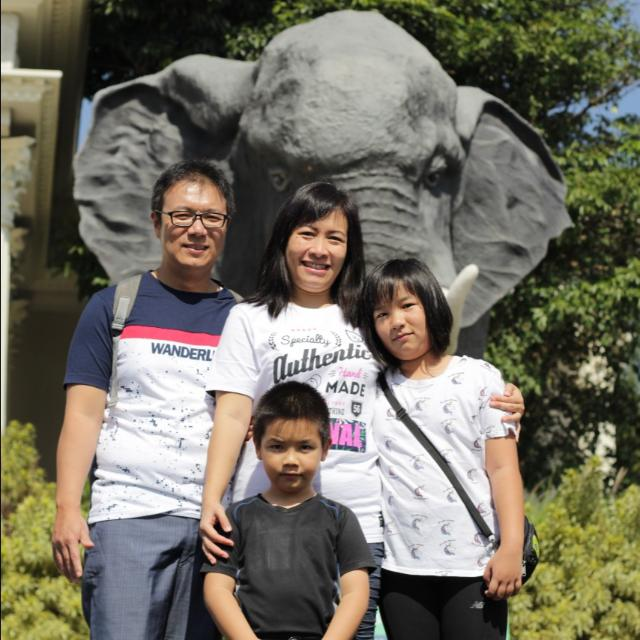
\includegraphics[scale=.35]{family}
\end{frame}

\begin{frame}{Outline}
  \tableofcontents
  % You might wish to add the option [pausesections]
\end{frame}


% Structuring a talk is a difficult task and the following structure
% may not be suitable. Here are some rules that apply for this
% solution: 

% - Exactly two or three sections (other than the summary).
% - At *most* three subsections per section.
% - Talk about 30s to 2min per frame. So there should be between about
%   15 and 30 frames, all told.

% - A conference audience is likely to know very little of what you
%   are going to talk about. So *simplify*!
% - In a 20min talk, getting the main ideas across is hard
%   enough. Leave out details, even if it means being less precise than
%   you think necessary.
% - If you omit details that are vital to the proof/implementation,
%   just say so once. Everybody will be happy with that.

%\begin{frame}{Make Titles Informative. Use Uppercase Letters.}{Subtitles are optional.}


\section{Apa Kata Alkitab?}
\begin{frame}{Apa kata Alkitab? (1/2)}
 	\emph{Pembacaan Alkitab}
	\begin{itemize}
		\item \textbf{Kejadian 2:18}\\
		TUHAN Allah berfirman: "\textit{Tidak baik, kalau manusia itu seorang diri saja. Aku akan menjadikan penolong baginya, yang sepadan dengan dia.}"
	\end{itemize}
	
	\begin{center}
		
\includegraphics[scale=.25]{my-other-half}
	\end{center}
\end{frame}

\begin{frame}{Apa kata Alkitab? (2/2)}
 	\emph{Pembacaan Alkitab}
	\begin{itemize}
		\item \textbf{Efesus 5:22-23} \\
		\textit{Kasih Kristus adalah dasar hidup suami isteri}
				
		\bigskip
		
		Hai isteri, tunduklah kepada suamimu seperti kepada Tuhan, karena suami adalah kepala isteri sama seperti Kristus adalah kepala jemaat. Dialah yang menyelamatkan tubuh.
	\end{itemize}
	\begin{center}
		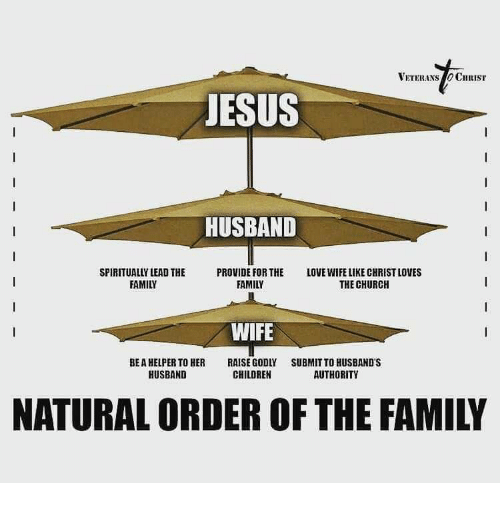
\includegraphics[scale=.275]{natural-order-in-a-family}	
	\end{center}	
\end{frame}


\section{Natur yang Berbeda}
\begin{frame}{Memahami natur yang berbeda antara pria dan wanita (1/23)}
		\textbf{Kejadian 3:16-19} \\
Firman-Nya kepada perempuan itu: "\textit{Susah payahmu waktu mengandung akan Kubuat sangat banyak; dengan kesakitan engkau akan melahirkan anakmu; namun engkau akan berahi kepada suamimu dan ia akan berkuasa atasmu.}" Lalu firman-Nya kepada manusia itu: "Karena engkau mendengarkan perkataan isterimu dan memakan dari buah pohon, yang telah Kuperintahkan kepadamu: Jangan makan dari padanya, maka \textit{terkutuklah tanah karena engkau; dengan bersusah payah engkau akan mencari rezekimu dari tanah seumur hidupmu: semak duri dan rumput duri yang akan dihasilkannya bagimu, dan tumbuh-tumbuhan di padang akan menjadi makananmu; dengan berpeluh engkau akan mencari makananmu, sampai engkau kembali lagi menjadi tanah, karena dari situlah engkau diambil; sebab engkau debu dan engkau akan kembali menjadi debu.}"
\end{frame}

\begin{frame}{Memahami natur yang berbeda antara pria dan wanita (2/23)}
	\begin{itemize}		
		\item Keadaan fisik pria $\Longrightarrow$ pria mengerjakan hal-hal yang memang \textbf{lebih membutuhkan kekuatan fisik}.
		
		\bigskip

		\item  Pria mengelola bumi dan mendapatkan makanan melalui tenaga yang diperasnya.
		
		\bigskip
		
		\item Wanita mendapatkan pemuasan batinnya melalui kesakitan pada saat ia melahirkan anaknya dan ketergantungannya pada suami.				
	\end{itemize}
\end{frame}

\begin{frame}{Memahami natur yang berbeda antara pria dan wanita (3/23)}
\emph{Yusuf} (\textbf{Matius 1:18-20}): Kelahiran Yesus Kristus adalah seperti berikut: Pada waktu Maria, ibu-Nya, bertunangan dengan Yusuf, ternyata ia mengandung dari Roh Kudus, sebelum mereka hidup sebagai suami isteri. Karena Yusuf suaminya, \textit{seorang yang tulus hati dan tidak mau mencemarkan nama isterinya di muka umum, ia bermaksud menceraikannya dengan diam-diam}. Tetapi ketika ia mempertimbangkan maksud itu, malaikat Tuhan nampak kepadanya dalam mimpi dan berkata: "Yusuf, anak Daud, janganlah engkau takut mengambil Maria sebagai isterimu, sebab anak yang di dalam kandungannya adalah dari Roh Kudus. 		
\end{frame}


\begin{frame}{Memahami natur yang berbeda antara pria dan wanita (4/23)}
\emph{Maria} (\textbf{Lukas 1:38}): Kata Maria: "\textit{Sesungguhnya aku ini adalah hamba Tuhan; jadilah padaku menurut perkataanmu itu.}" Lalu malaikat itu meninggalkan dia.
\end{frame}

\begin{frame}{Memahami natur yang berbeda antara pria dan wanita (5/23)}
\emph{Maria} (\textbf{Lukas 1:46-54}): Lalu kata Maria: "Jiwaku memuliakan Tuhan, dan hatiku bergembira karena Allah, Juruselamatku sebab Ia telah memperhatikan kerendahan hamba-Nya. Sesungguhnya, mulai dari sekarang segala keturunan akan menyebut aku berbahagia, karena Yang Mahakuasa telah melakukan perbuatan-perbuatan besar kepadaku dan nama-Nya adalah kudus. Dan rahmat-Nya turun-temurun atas orang yang takut akan Dia. Ia memperlihatkan kuasa-Nya dengan perbuatan tangan-Nya dan mencerai-beraikan orang-orang yang congkak hatinya; Ia menurunkan orang-orang yang berkuasa dari takhtanya dan meninggikan orang-orang yang rendah; Ia melimpahkan segala yang baik kepada orang yang lapar, dan menyuruh orang yang kaya pergi dengan tangan hampa; Ia menolong Israel, hamba-Nya, karena Ia mengingat rahmat-Nya, seperti yang dijanjikan-Nya kepada nenek moyang kita, kepada Abraham dan keturunannya untuk selama-lamanya." 	
\end{frame}

\begin{frame}{Memahami natur yang berbeda antara pria dan wanita (6/23)}
		\begin{itemize}
		\item Pria dengan naturnya \textbf{yang lebih rasional cenderung menyelesaikan masalah secara praktis}, berbeda dengan wanita \textbf{yang cenderung lebih mempercayai kerja emosinya}.
		
		\bigskip
		
		\textbf{Contoh}: Yusuf yang bereaksi secara rasional pada saat menemukan Maria, tunangannya yang mengandung 


		\bigskip
		
		Maria bereaksi secara emosional atas berita sukacita yang malaikat sampaikan kepadanya.		
	\end{itemize}	
\end{frame}

\begin{frame}{Memahami natur yang berbeda antara pria dan wanita (7/23)}
	\textbf{Dalam pemenuhan dan pelampiasan kebutuhan seksual} \\
	\emph{Samson} (\textbf{Hakim-Hakim 14-16}):
	Ia pulang dan memberitahukan kepada ayahnya dan ibunya: "Di Timna aku melihat seorang gadis Filistin. Tolong, ambillah dia menjadi isteriku. Tetapi ayahnya dan ibunya berkata kepadanya: "Tidak adakah di antara anak-anak perempuan sanak saudaramu atau di antara seluruh bangsa kita seorang perempuan, sehingga engkau pergi mengambil isteri dari orang Filistin, orang-orang yang tidak bersunat itu?" Tetapi jawab Simson kepada ayahnya: "Ambillah dia bagiku, sebab dia kusukai." \\
	$\cdots$ \\
		$\cdots$ \\
			$\cdots$ \\
	Sesudah itu Simson jatuh cinta kepada seorang perempuan dari lembah Sorek yang namanya Delila.
\end{frame}

\begin{frame}{Memahami natur yang berbeda antara pria dan wanita (8/23)}
	\emph{Daud} \textbf{(2 Samuel 11)}: Pada pergantian tahun, pada waktu raja-raja biasanya maju berperang, maka Daud menyuruh Yoab maju beserta orang-orangnya dan seluruh orang Israel. Mereka memusnahkan bani Amon dan mengepung kota Raba, sedang Daud sendiri tinggal di Yerusalem. Sekali peristiwa pada waktu petang, ketika Daud bangun dari tempat pembaringannya, lalu berjalan-jalan di atas sotoh istana, tampak kepadanya dari atas sotoh itu seorang perempuan sedang mandi; perempuan itu sangat elok rupanya. Lalu Daud menyuruh orang bertanya tentang perempuan itu dan orang berkata: "Itu adalah Batsyeba binti Eliam, isteri Uria orang Het itu." Sesudah itu Daud menyuruh orang mengambil dia. Perempuan itu datang kepadanya, lalu Daud tidur dengan dia. Perempuan itu baru selesai membersihkan diri dari kenajisannya. Kemudian pulanglah perempuan itu ke rumahnya.	
\end{frame}

\begin{frame}{Memahami natur yang berbeda antara pria dan wanita (9/23)}
	\emph{Amnon} \textbf{(2 Samuel 13)}:  Sesudah itu terjadilah yang berikut. Absalom bin Daud mempunyai seorang adik perempuan yang cantik, namanya Tamar; dan Amnon bin Daud jatuh cinta kepadanya. Hati Amnon sangat tergoda, sehingga ia jatuh sakit karena Tamar, saudaranya itu, sebab anak perempuan itu masih perawan dan menurut anggapan Amnon mustahil untuk melakukan sesuatu terhadap dia. Amnon mempunyai seorang sahabat bernama Yonadab, anak Simea kakak Daud. Yonadab itu seorang yang sangat cerdik. 13:4 Katanya kepada Amnon: "Hai anak raja, mengapa engkau demikian merana setiap pagi? Tidakkah lebih baik engkau memberitahukannya kepadaku?" Kata Amnon kepadanya: "Aku cinta kepada Tamar, adik perempuan Absalom, saudaraku itu." 
\end{frame}

\begin{frame}{Memahami natur yang berbeda antara pria dan wanita (10/23)}
Lalu berkatalah Yonadab kepadanya: "Berbaringlah di tempat tidurmu dan berbuat pura-pura sakit. Apabila ayahmu datang menengok engkau, maka haruslah engkau berkata kepadanya: Izinkanlah adikku Tamar datang memberi aku makan. Apabila ia menyediakan makanan di depan mataku, sehingga aku dapat melihatnya, maka aku akan memakannya dari tangannya." Sesudah itu berbaringlah Amnon dan berbuat pura-pura sakit. Ketika raja datang menengok dia, berkatalah Amnon kepada raja: "Izinkanlah adikku Tamar datang membuat barang dua kue di depan mataku, supaya aku memakannya dari tangannya." Lalu Daud menyuruh orang kepada Tamar, ke rumahnya, dengan pesan: "Pergilah ke rumah Amnon, kakakmu dan sediakanlah makanan baginya." Maka Tamar pergi ke rumah Amnon, kakaknya, yang sedang berbaring-baring, lalu anak perempuan itu mengambil adonan, meremasnya dan membuat kue di depan matanya, kemudian dibakarnya kue itu. Sesudah itu gadis itu mengambil kuali dan mengeluarkan isinya di depan Amnon, tetapi ia tidak mau makan. 	
\end{frame}

\begin{frame}{Memahami natur yang berbeda antara pria dan wanita (11/23)}
Berkatalah Amnon: "Suruhlah setiap orang keluar meninggalkan aku." Lalu keluarlah setiap orang meninggalkan dia. Lalu berkatalah Amnon kepada Tamar: "Bawalah makanan itu ke dalam kamar, supaya aku memakannya dari tanganmu." Tamar mengambil kue yang disediakannya itu, lalu membawanya kepada Amnon, kakaknya, ke dalam kamar. Ketika gadis itu menghidangkannya kepadanya supaya ia makan, dipegangnyalah gadis itu dan berkata kepadanya: "Marilah tidur dengan aku, adikku." Tetapi gadis itu berkata kepadanya: "Tidak kakakku, jangan perkosa aku, sebab orang tidak berlaku seperti itu di Israel. Janganlah berbuat noda seperti itu. Dan aku, ke manakah kubawa kecemaranku? Dan engkau ini, engkau akan dianggap sebagai orang yang bebal di Israel. Oleh sebab itu, berbicaralah dengan raja, sebab ia tidak akan menolak memberikan aku kepadamu." Tetapi Amnon tidak mau mendengarkan perkataannya, dan sebab ia lebih kuat dari padanya, diperkosanyalah dia, lalu tidur dengan dia.	
\end{frame}

\begin{frame}{Memahami natur yang berbeda antara pria dan wanita (12/23)}
\emph{Lea} \textbf{(Kejadian 30:14-21)}: Ketika Ruben pada musim menuai gandum pergi berjalan-jalan, didapatinyalah di padang buah dudaim, lalu dibawanya kepada Lea, ibunya. Kata Rahel kepada Lea: "Berilah aku beberapa buah dudaim yang didapat oleh anakmu itu." Jawab Lea kepadanya: "Apakah belum cukup bagimu mengambil suamiku? Sekarang pula mau mengambil lagi buah dudaim anakku?" Kata Rahel: "Kalau begitu biarlah ia tidur dengan engkau pada malam ini sebagai ganti buah dudaim anakmu itu." Ketika Yakub pada waktu petang datang dari padang, pergilah Lea mendapatkannya, sambil berkata: "Engkau harus singgah kepadaku malam ini, sebab memang engkau telah kusewa dengan buah dudaim anakku." Sebab itu tidurlah Yakub dengan Lea pada malam itu. Lalu Allah mendengarkan permohonan Lea. 
\end{frame}

\begin{frame}{Memahami natur yang berbeda antara pria dan wanita (13/23)}
Lea mengandung dan melahirkan anak laki-laki yang kelima bagi Yakub. Lalu kata Lea: "Allah telah memberi upahku, karena aku telah memberi budakku perempuan kepada suamiku." Maka ia menamai anak itu Isakhar. Kemudian Lea mengandung pula dan melahirkan anak laki-laki yang keenam bagi Yakub. Berkatalah Lea: "Allah telah memberikan hadiah yang indah kepadaku; sekali ini suamiku akan tinggal bersama-sama dengan aku, karena aku telah melahirkan enam orang anak laki-laki baginya." Maka ia menamai anak itu Zebulon. Sesudah itu ia melahirkan seorang anak perempuan dan menamai anak itu Dina. 	
\end{frame}

\begin{frame}{Memahami natur yang berbeda antara pria dan wanita (14/23)}
		\begin{itemize}
		\item Pria cenderung \textbf{memenuhi dan melampiaskan kebutuhan seksual secara instan dan semata-mata untuk kepuasan instingnya}, sehingga umumnya mereka dapat memisahkan antara cinta dan seks.
		
		\bigskip
		
		\textbf{Contoh}: Samson, Daud, Amnon 
		
		\bigskip
		
		\item \textbf{Bagi wanita, hubungan seksual tidak terpisahkan dari keterikatan emosinya}.
		
		\bigskip
		
		\textbf{Contoh}: Lea dan Tamar.
		
		\bigskip
		
		Hasil empiris juga menemukan bahwa perzinahan \\
		lebih banyak dilakukan oleh pria dibandingkan dengan wanita. 		
	\end{itemize}			
\end{frame}

\begin{frame}{Memahami natur yang berbeda antara pria dan wanita (15/23)}
	\textbf{Dalam orientasi hidup}\\
	\emph{Yakub} \textbf{(Kejadian 29)}: Laban mempunyai dua anak perempuan; yang lebih tua namanya Lea dan yang lebih muda namanya Rahel. Lea tidak berseri matanya, tetapi Rahel itu elok sikapnya dan cantik parasnya. Yakub cinta kepada Rahel, sebab itu ia berkata: "Aku mau bekerja padamu tujuh tahun lamanya untuk mendapat Rahel, anakmu yang lebih muda itu." Sahut Laban: "Lebih baiklah ia kuberikan kepadamu dari pada kepada orang lain; maka tinggallah padaku." Jadi bekerjalah Yakub tujuh tahun lamanya untuk mendapat Rahel itu, tetapi yang tujuh tahun itu dianggapnya seperti beberapa hari saja, karena cintanya kepada Rahel. 
\end{frame}

\begin{frame}{Memahami natur yang berbeda antara pria dan wanita (16/23)}
	Sesudah itu berkatalah Yakub kepada Laban: "Berikanlah kepadaku bakal isteriku itu, sebab jangka waktuku telah genap, supaya aku akan kawin dengan dia." Lalu Laban mengundang semua orang di tempat itu, dan mengadakan perjamuan. Tetapi pada waktu malam diambilnyalah Lea, anaknya, lalu dibawanya kepada Yakub. Maka Yakubpun menghampiri dia. Lagipula Laban memberikan Zilpa, budaknya perempuan, kepada Lea, anaknya itu, menjadi budaknya. Tetapi pada waktu pagi tampaklah bahwa itu Lea! Lalu berkatalah Yakub kepada Laban: "Apakah yang kauperbuat terhadap aku ini? Bukankah untuk mendapat Rahel aku bekerja padamu? Mengapa engkau menipu aku?" 
\end{frame}

\begin{frame}{Memahami natur yang berbeda antara pria dan wanita (17/23)}
	Jawab Laban: "Tidak biasa orang berbuat demikian di tempat kami ini, mengawinkan adiknya lebih dahulu dari pada kakaknya. Genapilah dahulu tujuh hari perkawinanmu dengan anakku ini; kemudian anakku yang lainpun akan diberikan kepadamu sebagai upah, asal engkau bekerja pula padaku tujuh tahun lagi." Maka Yakub berbuat demikian; ia menggenapi ketujuh hari perkawinannya dengan Lea, kemudian Laban memberikan kepadanya Rahel, anaknya itu, menjadi isterinya. Lagipula Laban memberikan Bilha, budaknya perempuan, kepada Rahel, anaknya itu, menjadi budaknya. Yakub menghampiri Rahel juga, malah ia lebih cinta kepada Rahel dari pada kepada Lea. Demikianlah ia bekerja pula pada Laban tujuh tahun lagi.
\end{frame}

\begin{frame}{Memahami natur yang berbeda antara pria dan wanita (18/23)}
\emph{Pemuda yang kaya} \textbf{(Matius 19)}: Ada seorang datang kepada Yesus, dan berkata: "Guru, perbuatan baik apakah yang harus kuperbuat untuk memperoleh hidup yang kekal?" Jawab Yesus: "Apakah sebabnya engkau bertanya kepada-Ku tentang apa yang baik? Hanya Satu yang baik. Tetapi jikalau engkau ingin masuk ke dalam hidup, turutilah segala perintah Allah." Kata orang itu kepada-Nya: "Perintah yang mana?" Kata Yesus: "Jangan membunuh, jangan berzinah, jangan mencuri, jangan mengucapkan saksi dusta, hormatilah ayahmu dan ibumu dan kasihilah sesamamu manusia seperti dirimu sendiri." Kata orang muda itu kepada-Nya: "Semuanya itu telah kuturuti, apa lagi yang masih kurang?" 	
\end{frame}

\begin{frame}{Memahami natur yang berbeda antara pria dan wanita (19/23)}
	Kata Yesus kepadanya: "Jikalau engkau hendak sempurna, pergilah, juallah segala milikmu dan berikanlah itu kepada orang-orang miskin, maka engkau akan beroleh harta di sorga, kemudian datanglah ke mari dan ikutlah Aku." Ketika orang muda itu mendengar perkataan itu, pergilah ia dengan sedih, sebab banyak hartanya. Yesus berkata kepada murid-murid-Nya: "Aku berkata kepadamu, sesungguhnya sukar sekali bagi seorang kaya untuk masuk ke dalam Kerajaan Sorga. Sekali lagi Aku berkata kepadamu, lebih mudah seekor unta masuk melalui lobang jarum dari pada seorang kaya masuk ke dalam Kerajaan Allah."
\end{frame}

\begin{frame}{Memahami natur yang berbeda antara pria dan wanita (20/23)}

	\begin{itemize}
		\item Pria lebih cenderung \textbf{memiliki orientasi hidup pada target dan upaya pencapaiannya} (\textit{target-oriented}).
		
		\bigskip
		
		\textbf{Contoh}: Yakub dan pemuda yang kaya.
						
	\end{itemize}	
\end{frame}

\begin{frame}{Memahami natur yang berbeda antara pria dan wanita (21/23)}
	\begin{itemize}
		\item \textbf{Orientasi wanita berubah pada saat kesempatan membina hubungan pribadi itu terbuka} (\textit{relational-oriented}).
		
		\bigskip		
		
		\textbf{Contoh}: Rut dan Maria saudara Lazarus (Yohanes 12:1-8).		
	\end{itemize}
\end{frame}

\begin{frame}{Memahami natur yang berbeda antara pria dan wanita (22/23)}
	\emph{Rut} \textbf{(Rut 1:16-17)}: Tetapi kata Rut: "Janganlah desak aku meninggalkan engkau dan pulang dengan tidak mengikuti engkau; sebab ke mana engkau pergi, ke situ jugalah aku pergi, dan di mana engkau bermalam, di situ jugalah aku bermalam: bangsamulah bangsaku dan Allahmulah Allahku; di mana engkau mati, akupun mati di sana, dan di sanalah aku dikuburkan. Beginilah kiranya TUHAN menghukum aku, bahkan lebih lagi dari pada itu, jikalau sesuatu apapun memisahkan aku dari engkau, selain dari pada maut!"
\end{frame}

\begin{frame}{Memahami natur yang berbeda antara pria dan wanita (23/23)}
	\emph{Maria saudara Lazarus} \textbf{(Yohanes 12:1-8)}: Enam hari sebelum Paskah Yesus datang ke Betania, tempat tinggal Lazarus yang dibangkitkan Yesus dari antara orang mati. Di situ diadakan perjamuan untuk Dia dan Marta melayani, sedang salah seorang yang turut makan dengan Yesus adalah Lazarus. Maka Maria mengambil setengah kati minyak narwastu murni yang mahal harganya, lalu meminyaki kaki Yesus dan menyekanya dengan rambutnya; dan bau minyak semerbak di seluruh rumah itu.	
\end{frame}

\section{Peran yang Diberikan Allah}
\begin{frame}{Memahami peran yang Allah berikan bagi suami dan istri Kristen (1/12)}
	\textbf{Sebagai suami}:
	\begin{itemize}
		\item pria dipanggil untuk menjadi \textbf{kepala keluarga} (Kejadian 2:18, Efesus 5:22-23, 1 Petrus 3:1-7)
	\end{itemize}
	\bigskip
	\textbf{Kejadian 2:18}: TUHAN Allah berfirman: "Tidak baik, kalau manusia itu seorang diri saja. Aku akan menjadikan penolong baginya, yang sepadan dengan dia. \\
	\textbf{Efesus 5:22-23}: Hai isteri, tunduklah kepada suamimu seperti kepada Tuhan, karena suami adalah kepala isteri sama seperti Kristus adalah kepala jemaat. Dialah yang menyelamatkan tubuh.
\end{frame}

\begin{frame}{Memahami peran yang Allah berikan bagi suami dan istri Kristen (2/12)}
	\textbf{1 Petrus 3:1-7}: \emph{Hidup bersama suami isteri} \\
	Demikian juga kamu, hai isteri-isteri, tunduklah kepada suamimu, supaya jika ada di antara mereka yang tidak taat kepada Firman, mereka juga tanpa perkataan dimenangkan oleh kelakuan isterinya, jika mereka melihat, bagaimana murni dan salehnya hidup isteri mereka itu. Perhiasanmu janganlah secara lahiriah, yaitu dengan mengepang-ngepang rambut, memakai perhiasan emas atau dengan mengenakan pakaian yang indah-indah, tetapi perhiasanmu ialah manusia batiniah yang tersembunyi dengan perhiasan yang tidak binasa yang berasal dari roh yang lemah lembut dan tenteram, yang sangat berharga di mata Allah. 
\end{frame}

\begin{frame}{Memahami peran yang Allah berikan bagi suami dan istri Kristen (3/12)}
Sebab demikianlah caranya perempuan-perempuan kudus dahulu berdandan, yaitu perempuan-perempuan yang menaruh pengharapannya kepada Allah; mereka tunduk kepada suaminya, sama seperti Sara taat kepada Abraham dan menamai dia tuannya. Dan kamu adalah anak-anaknya, jika kamu berbuat baik dan tidak takut akan ancaman. Demikian juga kamu, hai suami-suami, hiduplah bijaksana dengan isterimu, sebagai kaum yang lebih lemah! Hormatilah mereka sebagai teman pewaris dari kasih karunia, yaitu kehidupan, supaya doamu jangan terhalang.  	
\end{frame}

\begin{frame}{Memahami peran yang Allah berikan bagi suami dan istri Kristen (4/12)}
	\textbf{Sebagai suami}:
	\begin{itemize}
		\item Sebagai kepala keluarga, ia dipanggil untuk meneladani Yesus yang menyangkal diri-Nya demi kepentingan orang yang dikasihi-Nya. \\
		Prinsip kepemimpinan yang dimulai dengan memperhambakan dirinya sendiri (Markus 10:43-44) $\Longrightarrow$ menempatkan pria dalam posisi \textit{leading servant}.											
	\end{itemize}

	\bigskip	
	
	\textbf{Markus 10:43-44}: Tidaklah demikian di antara kamu. Barangsiapa ingin menjadi besar di antara kamu, hendaklah ia menjadi \textit{pelayan}mu, dan barangsiapa ingin menjadi yang terkemuka di antara kamu, hendaklah ia menjadi \textit{hamba} untuk semuanya.
\end{frame}

\begin{frame}{Memahami peran yang Allah berikan bagi suami dan istri Kristen (5/12)}
	\textbf{Sebagai istri}:
	\begin{itemize}
		\item Sebagai penolong yang sepadan, wanita juga dipanggil untuk meneladani Kristus dalam bentuk \textbf{kerelaan untuk tunduk} (\textit{submissive}) dan menghormati suami. \\
		\textbf{Sarah} (1 Petrus 3:1-7) dan \textbf{perempuan-perempuan yang saleh di PL} (2 Raja-Raja 4:8-37, Amsal 31:10-31).
		\item Sikap ini hanya dimiliki oleh \textbf{wanita-wanita yang mencintai Tuhan} dan \textbf{rela menyangkal dirinya sendiri}. \\
		Melalui merekalah, Allah berkarya sehingga kehadiran wanita-wanita tersebut \textbf{mengubah dan memperbaharui suami dan seluruh keluarganya} (1 Petrus 3:1-5).		
	\end{itemize}
\end{frame}

\begin{frame}{Memahami peran yang Allah berikan bagi suami dan istri Kristen (6/12)}
	\textbf{2 Raja-Raja 4:8-37}: \textbf{Perempuan Sunem dengan anaknya} \\
	Pada suatu hari Elisa pergi ke Sunem. Di sana tinggal seorang perempuan kaya yang mengundang dia makan. Dan seberapa kali ia dalam perjalanan, singgahlah ia ke sana untuk makan. Berkatalah perempuan itu kepada suaminya: "Sesungguhnya aku sudah tahu bahwa orang yang selalu datang kepada kita itu adalah abdi Allah yang kudus. Baiklah kita membuat sebuah kamar atas yang kecil yang berdinding batu, dan baiklah kita menaruh di sana baginya sebuah tempat tidur, sebuah meja, sebuah kursi dan sebuah kandil, maka apabila ia datang kepada kita, ia boleh masuk ke sana."  \\
	$\cdots$ \\
	$\cdots$
\end{frame}

\begin{frame}{Memahami peran yang Allah berikan bagi suami dan istri Kristen (7/12)}
	Kemudian berkatalah Elisa: "Apakah yang dapat kuperbuat baginya?" Jawab Gehazi: "Ah, ia tidak mempunyai anak, dan suaminya sudah tua." Lalu berkatalah Elisa: "Panggillah dia!" Dan sesudah dipanggilnya, berdirilah perempuan itu di pintu. Berkatalah Elisa: "Pada waktu seperti ini juga, tahun depan, engkau ini akan menggendong seorang anak laki-laki." Tetapi jawab perempuan itu: "Janganlah tuanku, ya abdi Allah, janganlah berdusta kepada hambamu ini!" Mengandunglah perempuan itu, lalu melahirkan seorang anak laki-laki pada waktu seperti itu juga, pada tahun berikutnya, seperti yang dikatakan Elisa kepadanya. \\
	$\cdots$ \\
	$\cdots$ 
\end{frame}

\begin{frame}{Memahami peran yang Allah berikan bagi suami dan istri Kristen (8/12)}
Diangkatnyalah dia, dibawanya pulang kepada ibunya. Duduklah dia di pangkuan ibunya sampai tengah hari, tetapi sesudah itu matilah dia. Lalu naiklah perempuan itu, dibaringkannyalah dia di atas tempat tidur abdi Allah itu, ditutupnyalah pintu dan pergi, sehingga anak itu saja di dalam kamar.	\\
	$\cdots$ \\
	$\cdots$ \\
Lalu berkatalah perempuan itu: "Adakah kuminta seorang anak laki-laki dari pada tuanku? Bukankah telah kukatakan: Jangan aku diberi harapan kosong?" 	
\end{frame}

\begin{frame}{Memahami peran yang Allah berikan bagi suami dan istri Kristen (9/12)}
Maka berkatalah Elisa kepada Gehazi: "Ikatlah pinggangmu, bawalah tongkatku di tanganmu dan pergilah. Apabila engkau bertemu dengan seseorang, janganlah beri salam kepadanya dan apabila seseorang memberi salam kepadamu, janganlah balas dia, kemudian taruhlah tongkatku ini di atas anak itu." Tetapi berkatalah ibu anak itu: "Demi TUHAN yang hidup dan demi hidupmu sendiri, sesungguhnya aku tidak akan meninggalkan engkau."	\\
	$\cdots$ \\
	$\cdots$ \\
 Maka bersinlah anak itu sampai tujuh kali, lalu membuka matanya. Kemudian Elisa memanggil Gehazi dan berkata: "Panggillah perempuan Sunem itu!" Dipanggilnyalah dia, lalu datanglah ia kepadanya, maka berkatalah Elisa: "Angkatlah anakmu ini!" Masuklah perempuan itu, lalu tersungkur di depan kaki Elisa dan sujud menyembah dengan mukanya sampai ke tanah. Kemudian diangkatnyalah anaknya, lalu keluar.				
\end{frame}

\begin{frame}{Memahami peran yang Allah berikan bagi suami dan istri Kristen (10/12)}
		\textbf{Amsal 31:10-31}: Isteri yang cakap siapakah akan mendapatkannya? Ia lebih berharga dari pada permata. Hati suaminya percaya kepadanya, suaminya tidak akan kekurangan keuntungan. Ia berbuat baik kepada suaminya dan tidak berbuat jahat sepanjang umurnya. Ia mencari bulu domba dan rami, dan senang bekerja dengan tangannya. Ia serupa kapal-kapal saudagar, dari jauh ia mendatangkan makanannya. Ia bangun kalau masih malam, lalu menyediakan makanan untuk seisi rumahnya, dan membagi-bagikan tugas kepada pelayan-pelayannya perempuan. Ia membeli sebuah ladang yang diingininya, dan dari hasil tangannya kebun anggur ditanaminya. Ia mengikat pinggangnya dengan kekuatan, ia menguatkan lengannya. Ia tahu bahwa pendapatannya menguntungkan, pada malam hari pelitanya tidak padam. 
\end{frame}

\begin{frame}{Memahami peran yang Allah berikan bagi suami dan istri Kristen (11/12)}
Tangannya ditaruhnya pada jentera, jari-jarinya memegang pemintal. Ia memberikan tangannya kepada yang tertindas, mengulurkan tangannya kepada yang miskin. Ia tidak takut kepada salju untuk seisi rumahnya, karena seluruh isi rumahnya berpakaian rangkap. Ia membuat bagi dirinya permadani, lenan halus dan kain ungu pakaiannya. Suaminya dikenal di pintu gerbang, kalau ia duduk bersama-sama para tua-tua negeri. Ia membuat pakaian dari lenan, dan menjualnya, ia menyerahkan ikat pinggang kepada pedagang. Pakaiannya adalah kekuatan dan kemuliaan, ia tertawa tentang hari depan. Ia membuka mulutnya dengan hikmat, pengajaran yang lemah lembut ada di lidahnya. 
\end{frame}

\begin{frame}{Memahami peran yang Allah berikan bagi suami dan istri Kristen (12/12)}
Ia mengawasi segala perbuatan rumah tangganya, makanan kemalasan tidak dimakannya. Anak-anaknya bangun, dan menyebutnya berbahagia, pula suaminya memuji dia: Banyak wanita telah berbuat baik, tetapi kau melebihi mereka semua. Kemolekan adalah bohong dan kecantikan adalah sia-sia, tetapi isteri yang takut akan TUHAN dipuji-puji. Berilah kepadanya bagian dari hasil tangannya, biarlah perbuatannya memuji dia di pintu-pintu gerbang!  				
\end{frame}

\section{7 Perbedaan Terbesar antara Saudara dengan Pasangan Saudara}
\begin{frame}{7 Perbedaan antara Lelaki dan Perempuan}
	\begin{columns}[c]		
		\column{1.5in}
		\begin{itemize}
			\item<2-> Fisik
			\hfill \break
			\item<3-> Uang
			\hfill \break
			\item<4-> Relasi
			\hfill \break
			\item<5-> Verbal
		\end{itemize}		
		\column{2.5in}
		\begin{itemize}
			\item<6-> Kebutuhan 
			\hfill \break
			\item<7-> Aktivitas
			\hfill \break
			\item<8-> Kasih Sayang
		\end{itemize}				
	\end{columns}
\end{frame}

\begin{frame}{Perbedaan mengenai Fisik (\textit{Physical})}
	\begin{itemize}
		\item<2-> Koneksi otak laki-laki dan perempuan yang berbeda.
		\hfill \break
		\item<3-> Laki-laki lebih dominan otak sebelah kiri (logika) dan perempuan lebih seimbang\footnote{https://www.allprodad.com/the-10-biggest-differences-between-you-and-your-wife}.
		\hfill \break
		\item<4-> Akibatnya, laki-laki cenderung fokus pada satu pekerjaan sampai selesai.
		\hfill \break		
		\item<5-> Sedangkan, perempuan dapat mengerjakan \textit{multiple tasks at a time, sometimes completing them or leaving them for a later}.
		\begin{center}
	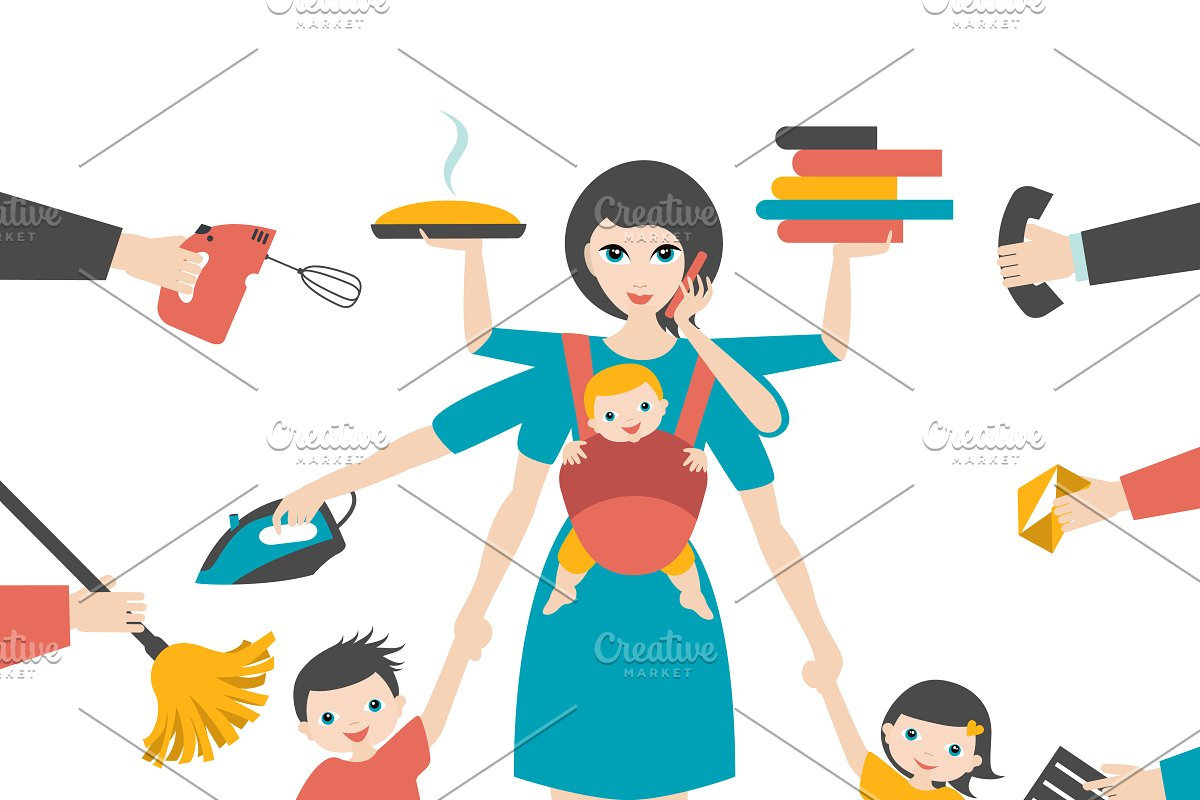
\includegraphics[scale=.1]{multitask-woman}			
		\end{center}
	\end{itemize}
\end{frame}

\begin{frame}{Perbedaan mengenai Pengeluaran (\textit{Money})}
	\begin{itemize}
		\item Laki-laki mengeluarkan uang untuk sesuatu yang mereka butuhkan.
		\hfill \break
		\item<2-> Umumnya perempuan akan membeli sesuatu yang mereka \textit{tidak} butuhkan jika ada \textit{sale}.
	\end{itemize}
\end{frame}

\begin{frame}{Perbedaan mengenai Relasi (\textit{Relationally})}
	\begin{itemize}
		\item<2-> Perempuan membangun hubungan dengan \textit{sharing emotions} sedangkan laki-laki \textit{sharing activities --- doing things together}.
		\hfill \break
		\item<3-> Menurut \citet{mayemotional2017}, perempuan \textit{lebih ekspresif dalam menampilkan emosi} dilihat dari raut muka.\\
		Ketika ada iklan lucu, lebih banyak perempuan yang senyum daripada laki-laki dan senyum perempuan lebih lama daripada laki-laki.
	\end{itemize}
\end{frame}

\begin{frame}{Perbedaan tentang Pengungkapan Lisan (\textit{Verbally})}
	\begin{itemize}
		\item<1-> Laki-laki $\Longrightarrow$ padat (\textit{concise}) dan bahasa pendek.
		\hfill \break
		\item<2-> Perempuan $\Longrightarrow$ panjang dan detil.
		\hfill \break
		\item<3-> \textit{Story} tentang Rachel dan Ross dari TV series "Friends".
	\end{itemize}
\end{frame}

\begin{frame}{\textit{Story} tentang Rachel dan Ross dari TV series "Friends"}
%	\includemedia[width=7.5cm, height=7.5cm, addresource=Difference-between-men-and-women.mp4, transparent, activate=pagevisible,
%	flashvars={
%		source=Difference-between-men-and-women.mp4 
%		&autoPlay=true
%		&loop=false
%	} ]{}{Difference-between-men-and-women.mp4}
	\begin{center}
	\movie[width=12cm,height=7cm,poster,autostart,showcontrols=<true>]{}{Difference-between-men-and-women.mp4}		
	\end{center}
\end{frame}

\begin{frame}{Perbedaan mengenai Kebutuhan (\textit{Needs})}
		\begin{itemize}
			\item Perempuan memiliki kebutuhan untuk \textit{didengar}.
			\hfill \break
			\item<2-> Hal ini dapat konflik dengan laki-laki yang lebih suka \textit{memberikan solusi} daripada \textit{mendengar}.
		\end{itemize}			
\end{frame}

%\begin{frame}{\textbf{Perbedaan mengenai Nilai (\textit{Values})}}
%	\begin{itemize}
%		\item<1-> Perempuan mungkin $\Rightarrow$ kerapihan (\textit{neatness}) dan keteraturan (\textit{order}).
%		\hfill \break
%		\item<2-> Laki-laki mungkin $\Rightarrow$ \textit{power} dan efisiensi.
%		\hfill \break
%		\item<3-> \textbf{Solusi}: idealnya, semakin lama menikah, nilai akan semakin menyatu.
%	\end{itemize}
%\end{frame}

\begin{frame}{Perbedaan mengenai Aktivitas (\textit{Activities})}\footnote{https://www.allprodad.com/10-creative-ways-spend-time-wife}
	\begin{itemize}
		\item<2-> \textit{Exercise together}.
		\hfill \break
		\item<3-> \textit{Sign up for a class together}.
		\hfill \break
		\item<4-> \textit{Volunteer together}.
		\hfill \break
		\item<5-> \textit{Take it in turns to organize a "mystery adventure date"}.
		\hfill \break
		\item<6-> \textit{Step out together down memory lane}.
	\end{itemize}
\end{frame}

\begin{frame}{Perbedaan mengenai \textit{Affection} (1/3)}
	\citet{chapman2015love} menjelaskan bahwa terdapat 5 bahasa kasih untuk mempertahankan cinta yang \textit{membara}.
	\begin{itemize}
		\item<2-> \emph{Words of Affirmation}. \\
		"\textit{My husband's encouraging words give me confidence}",\\
		"\textit{It makes me feel really good when my husband tells me he appreciates me}",\\
		"\textit{I love hearing my husband tell me that he missed me}".
		\hfill \break
		\item<3-> \emph{Quality Time}. \\
		"\textit{My husband doesn't interrupt me when I am talking, and I like that}", \\
		"\textit{It doesn't matter where we go, I just like going places with my husband}", \\
		"\textit{I love to watch movies with my husband}".
	\end{itemize}
\end{frame}

\begin{frame}{Perbedaan mengenai \textit{Affection} (2/3)}
	\citet{chapman2015love} menjelaskan bahwa terdapat 5 bahasa kasih untuk mempertahankan cinta yang \textit{membara}.
	\begin{itemize}
		\item<2-> \emph{Receiving Gifts}. \\
		"\textit{My husband lets me know he loves me by giving me gifts}", \\
		"\textit{I never get tired of receiving gifts from my husband}", \\
		"\textit{I love surprise gifts from my husband}".
		\hfill \break
		\item<3-> \emph{Acts of Service}. \\
		"\textit{My husband shows his love by helping me without me having to ask}",\\
		"\textit{My husband is good about asking how he can help when I'm tired}", \\
		"\textit{It means a lot to me when my husband helps me despite being busy}".		
	\end{itemize}
\end{frame}

\begin{frame}{Perbedaan mengenai \textit{Affection} (3/3)}
	\begin{itemize}
		\item<2-> \emph{Physical Touch}. \\
		"\textit{I love cuddling with my husband}", \\
		"\textit{I love it that my husband can't keep his hands off me}", \\
		"\textit{I love hugging and kissing my husband after we've been apart for a while}". \\			
	\end{itemize}
\end{frame}


\section{Difference Between Man and Woman by Dr. Chirag N. Patel}
\begin{frame}{Video: Difference Between Man and Woman (1/2)}
	Dr. Chirag N. Patel menjelaskan perbedaan laki-laki dan perempuan dari segi 
	\begin{itemize}
		\item pakaian (\textit{dress}), 
		\item \textit{sharing a bed}, 
		\item fokus, 
		\item cara berpikir, dan
		\item berbagai macam kebiasaan.
	\end{itemize}			
\end{frame}

\begin{frame}{Video: Difference Between Man and Woman (2/2)}
	\begin{center}
	\movie[width=12cm,height=7cm,poster,autostart,showcontrols=<true>]{}{Difference-Between-Man-and-Woman-I-Amazing-Facts.mp4}		
	\end{center}
\end{frame}

\section{Conclusion: Biblical View}
\begin{frame}{Conclusion}
	\begin{itemize}
		\item Pria sebagai Kepala Keluarga berarti \textit{man has a holy obligation before God to lay down his life for his wife, his children}.
		
		\bigskip		
				
		\item For a husband, it means that he has his wife's best interests at heart, that he sacrifices his own desires for hers, that he puts her first always in his affections. 
		
		\bigskip		
		
		\item For a wife, submission in this context means believing that God is able to work through her husband to accomplish HIS will in her life, to protect her interests, and to meet her deepest needs.
	\end{itemize}
\end{frame}

%\begin{frame}{Blocks}
%\begin{block}{Block Title}
%You can also highlight sections of your presentation in a block, with it's own title
%\end{block}
%\begin{theorem}
%There are separate environments for theorems, examples, definitions and proofs.
%\end{theorem}
%\begin{example}
%Here is an example of an example block.
%\end{example}
%\end{frame}


% All of the following is optional and typically not needed. 
%\appendix
%\section<presentation>*{\appendixname}
%\subsection<presentation>*{For Further Reading}
%
\begin{frame}[allowframebreaks]
  \frametitle<presentation>{\textbf{Referensi}}
    {\footnotesize
    \bibliographystyle{apalike}
    \bibliography{references}
    }    
\end{frame}

%\makeatletter % to change template
%    \setbeamertemplate{headline}[default] % not mandatory, but I though it was better to set it blank
%    \def\beamer@entrycode{\vspace*{-\headheight}} % here is the part we are interested in :)
%\makeatother

%\begin{frame}[plain]
%		\centering
\includegraphics[scale=0.5]{Logo-Maranatha-Untuk-Belakang-02}	
%\end{frame}

\begin{frame}[plain]
		\centering
\includegraphics[scale=1]{thank-you}	
		hendra.bunyamin@gmail.com
\end{frame}


\end{document}


